\section{Discussion}
\label{sec:discussion}

We synthesize findings across our four research questions to provide practical guidance for deploying synthetic kernel traces in real-world ML pipelines. Figure~\ref{fig:unified-landscape} summarizes key trends across workloads, model configurations, and evaluation dimensions.

\subsection{When Does Synthetic Trace Generation Work in Practice?}

Our results show that the utility of synthetic kernel traces is fundamentally workload-dependent. Deterministic, structured workloads benefit substantially more from synthetic augmentation than I/O-heavy, non-deterministic systems. The \texttt{scimark2} benchmark illustrates this clearly: at a context length of $L=4096$, synthetic augmentation achieves 87 hookup is near real-only performance (89.8\%), demonstrating that diffusion models can generate production-quality traces when execution patterns are stable and repetitive.

In contrast, I/O-intensive workloads such as \texttt{stream} and \texttt{iozone} exhibit significant degradation, even at long context lengths. These systems involve asynchronous interactions with filesystems and devices, where execution order and timing depend on external state that is not explicitly modeled (e.g., filesystem cache state, device queue depth, or network backpressure). As a result, diffusion models struggle to capture their inherent nondeterminism.

For practitioners, this distinction is critical. Synthetic augmentation is viable for compute-heavy, deterministic workloads and can meaningfully expand limited datasets. For I/O-dominated systems, synthetic traces should be used cautiously and primarily for non-critical tasks such as testing or exploratory analysis.

\subsection{Temporal Context Is the Primary Quality Driver}

Across all workloads, temporal context length emerges as the dominant factor affecting synthetic trace quality. Increasing context from $L=256$ to $L=4096$ yields an average improvement of +29.9 F1-macro points (+104\% relative), with every benchmark benefiting from longer context.

Longer context enables diffusion models to capture long-range execution dependencies that span hundreds or thousands of events, such as nested loops, phased computation, and recurring scheduling patterns. This effect is especially pronounced for structured workloads: for \texttt{scimark2}, longer context transforms synthetic traces from unusable (40.6\% F1 at $L=256$) to near-parity with real data (87.2\% at $L=4096$).

However, context length alone is not sufficient. While I/O-heavy workloads improve substantially with longer context, they do not reach production-level fidelity, indicating that additional modeling of external system state (e.g., filesystem caching, device queues, or asynchronous I/O effects) may be required. In our experimental setup, increasing context length from $L=256$ to $L=4096$ required approximately 16$\times$ more GPU memory and 4$\times$ longer training time, making quality gains beyond $L=4096$ increasingly expensive relative to their marginal benefit. This cost sensitivity highlights the practical trade-off exposed by RQ3 between temporal context and deployability.




\subsection{Constraint-Guided Repair as Engineering Best Practice}

Constraint-guided repair provides consistent, low-risk improvements across configurations. Although the average F1 gain is modest (+0.3\% to +4.3\%), repair delivers two critical benefits. First, it guarantees structural validity by enforcing correct event transitions, CPU affinity, and attribute consistency. This guarantee is essential for applications such as trace replay or debugging, where invalid traces are unacceptable.

Second, repair is most effective precisely when generative models are weakest. At shorter context lengths, where diffusion models produce more violations, repair yields the largest gains. At longer contexts, repair still provides incremental improvements with negligible overhead. Given its simplicity and safety guarantees, constraint-guided repair should be treated as a default component of any synthetic trace generation pipeline.

\subsection{Cost--Quality Trade-offs in Model Design}

Our ablation study reveals that simpler diffusion models can achieve nearly the same quality as feature-rich models at a fraction of the computational cost. A Base model using only event type and timing information achieves within 1--3\% of a Full six-channel model while requiring approximately three times fewer resources. For several workloads, the Base model even outperforms the Full configuration, suggesting that additional channels can introduce noise rather than useful signal.

Only highly structured workloads such as \texttt{scimark2} consistently benefit from richer feature sets, and even there the gains are marginal. These results support a tiered deployment strategy: start with a simple, low-cost model for most workloads, and selectively enable richer features only when the additional complexity is justified.

\subsection{Beyond Exact Prediction: Practical Value of Synthetic Traces}

While macro-F1 highlights limitations in rare-event modeling, secondary metrics reveal important practical value. Weighted F1 and accuracy remain high (86--97\%), and Top-$K$ accuracy consistently exceeds 96\%. This indicates that models trained on synthetic data capture common execution behavior and generate plausible alternative next events even when the top prediction is incorrect.

These properties enable several practical applications. Synthetic traces are well suited for software testing and fuzzing, where diverse plausible scenarios are more valuable than exact prediction. They facilitate privacy-preserving data sharing by preserving typical behavior without exposing sensitive details. They also support development and edge-case exploration when real production data is unavailable or expensive to collect.

\subsection{Implications for Future Systems}

Our findings suggest several directions for future work. Longer context lengths enabled by sparse attention mechanisms may further improve quality for challenging workloads. Workload-specific architectures could better model I/O-heavy systems by incorporating explicit representations of external state. Improved rare-event modeling techniques may reduce the gap between macro-F1 and overall accuracy. Finally, conditional generation could enable targeted synthesis of traces with specific properties, increasing usefulness for testing and analysis.

\subsection{When Synthetic Traces Are Not a Drop-In Replacement}
\label{subsec:failure-boundaries}

Despite strong performance on structured workloads, our results clearly indicate that \textsc{SynthTrace} is not a universal substitute for real kernel traces. For I/O-dominated workloads with high nondeterminism (e.g., \texttt{stream}, \texttt{iozone}), synthetic traces remain substantially less reliable, even at long context lengths ($L=4096$). In these settings, diffusion models struggle to capture asynchronous behavior arising from filesystem caching, device queues, and external latency sources.

As a result, practitioners should avoid relying on synthetic traces as a primary data source for safety-critical applications such as anomaly detection on rare I/O failures or security monitoring. Instead, synthetic traces are better suited as a complementary resource—for testing, development, or privacy-preserving analysis—where approximate behavior is acceptable and diversity is more important than exact fidelity.


\begin{figure}[t]
\centering
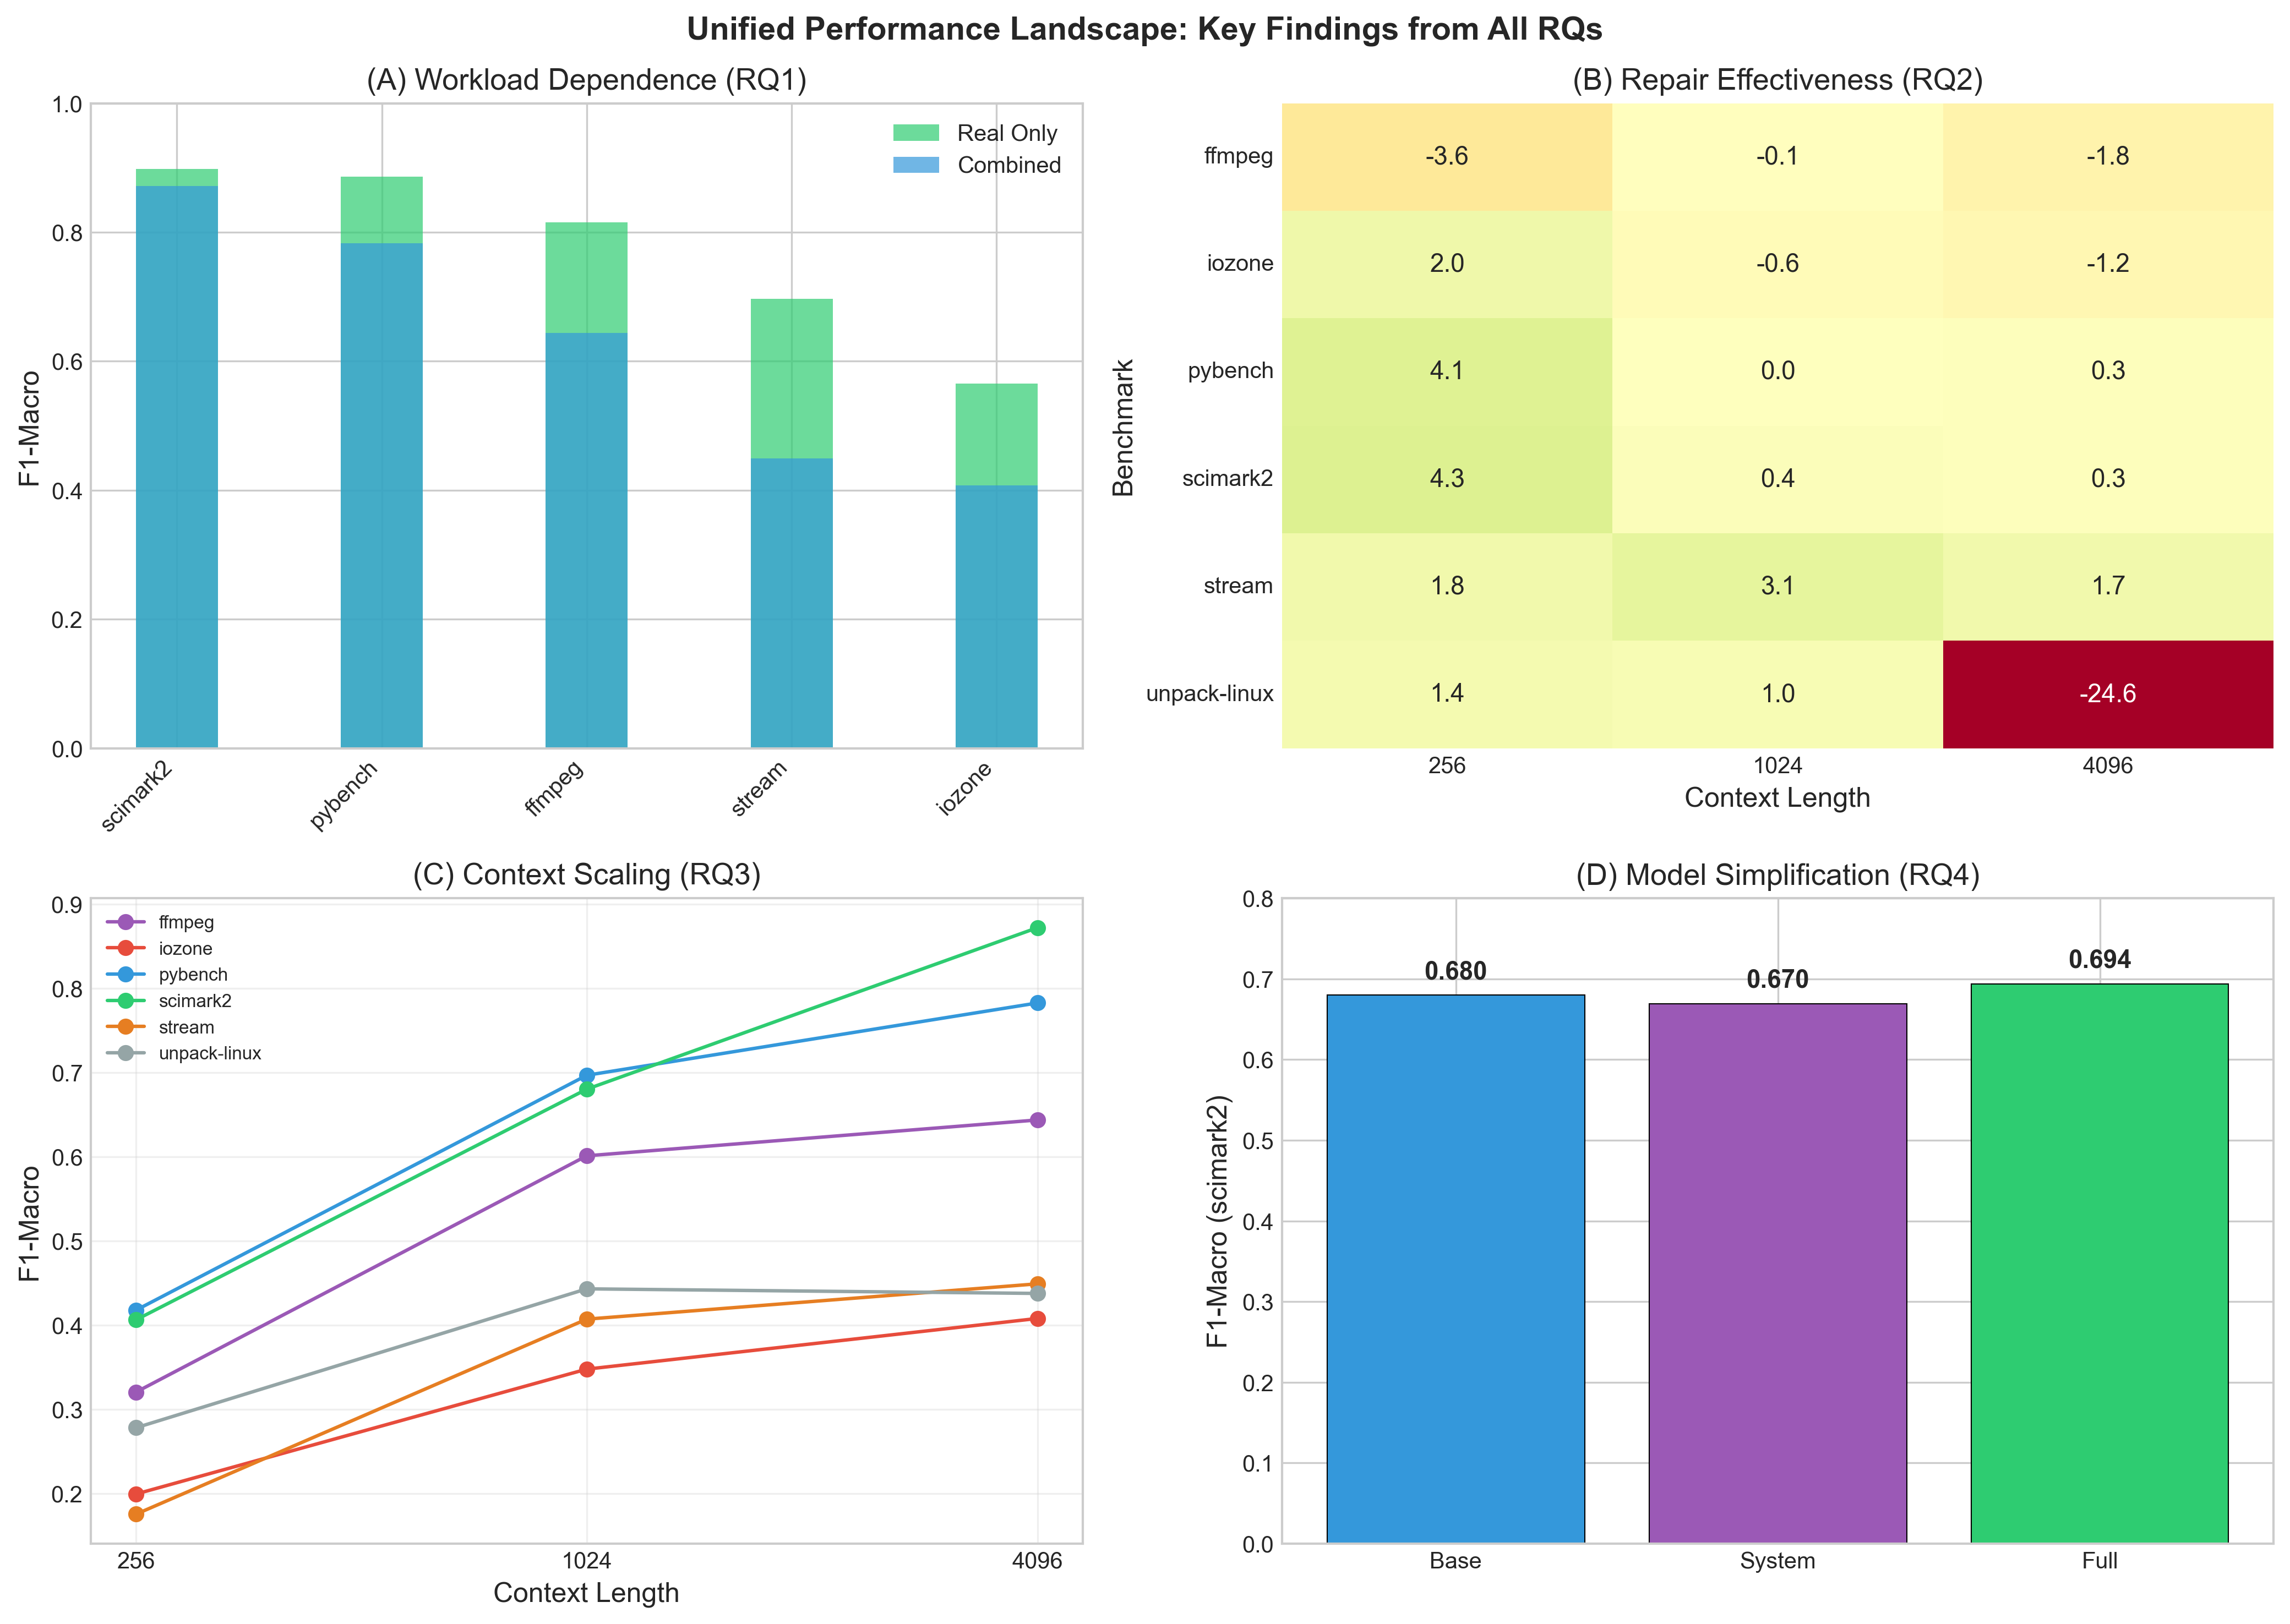
\includegraphics[width=0.95\columnwidth]{figures/cross_rq_plot12_unified_landscape.png}
\caption{Unified Performance Landscape showing key findings from all four research questions. (A) Workload Dependence (RQ1): scimark2 and pybench achieve near-parity with real data, while I/O-heavy workloads show significant degradation. (B) Repair Effectiveness (RQ2): Constraint-guided repair provides consistent improvements, especially at shorter context lengths. (C) Context Scaling (RQ3): All benchmarks benefit from longer context, with scimark2 showing +46.6\% improvement from L=256 to L=4096. (D) Model Simplification (RQ4): Base 2-channel model achieves 97\% of Full 6-channel performance for scimark2.}
\label{fig:unified-landscape}
\end{figure}



% \section{Discussion}
% \label{sec:discussion}

% We synthesize findings from our four research questions to provide actionable insights for practitioners and identify opportunities for future research. Figure~\ref{fig:unified-landscape} provides a comprehensive overview of key findings across all RQs.

% \begin{figure}[t]
% \centering
% 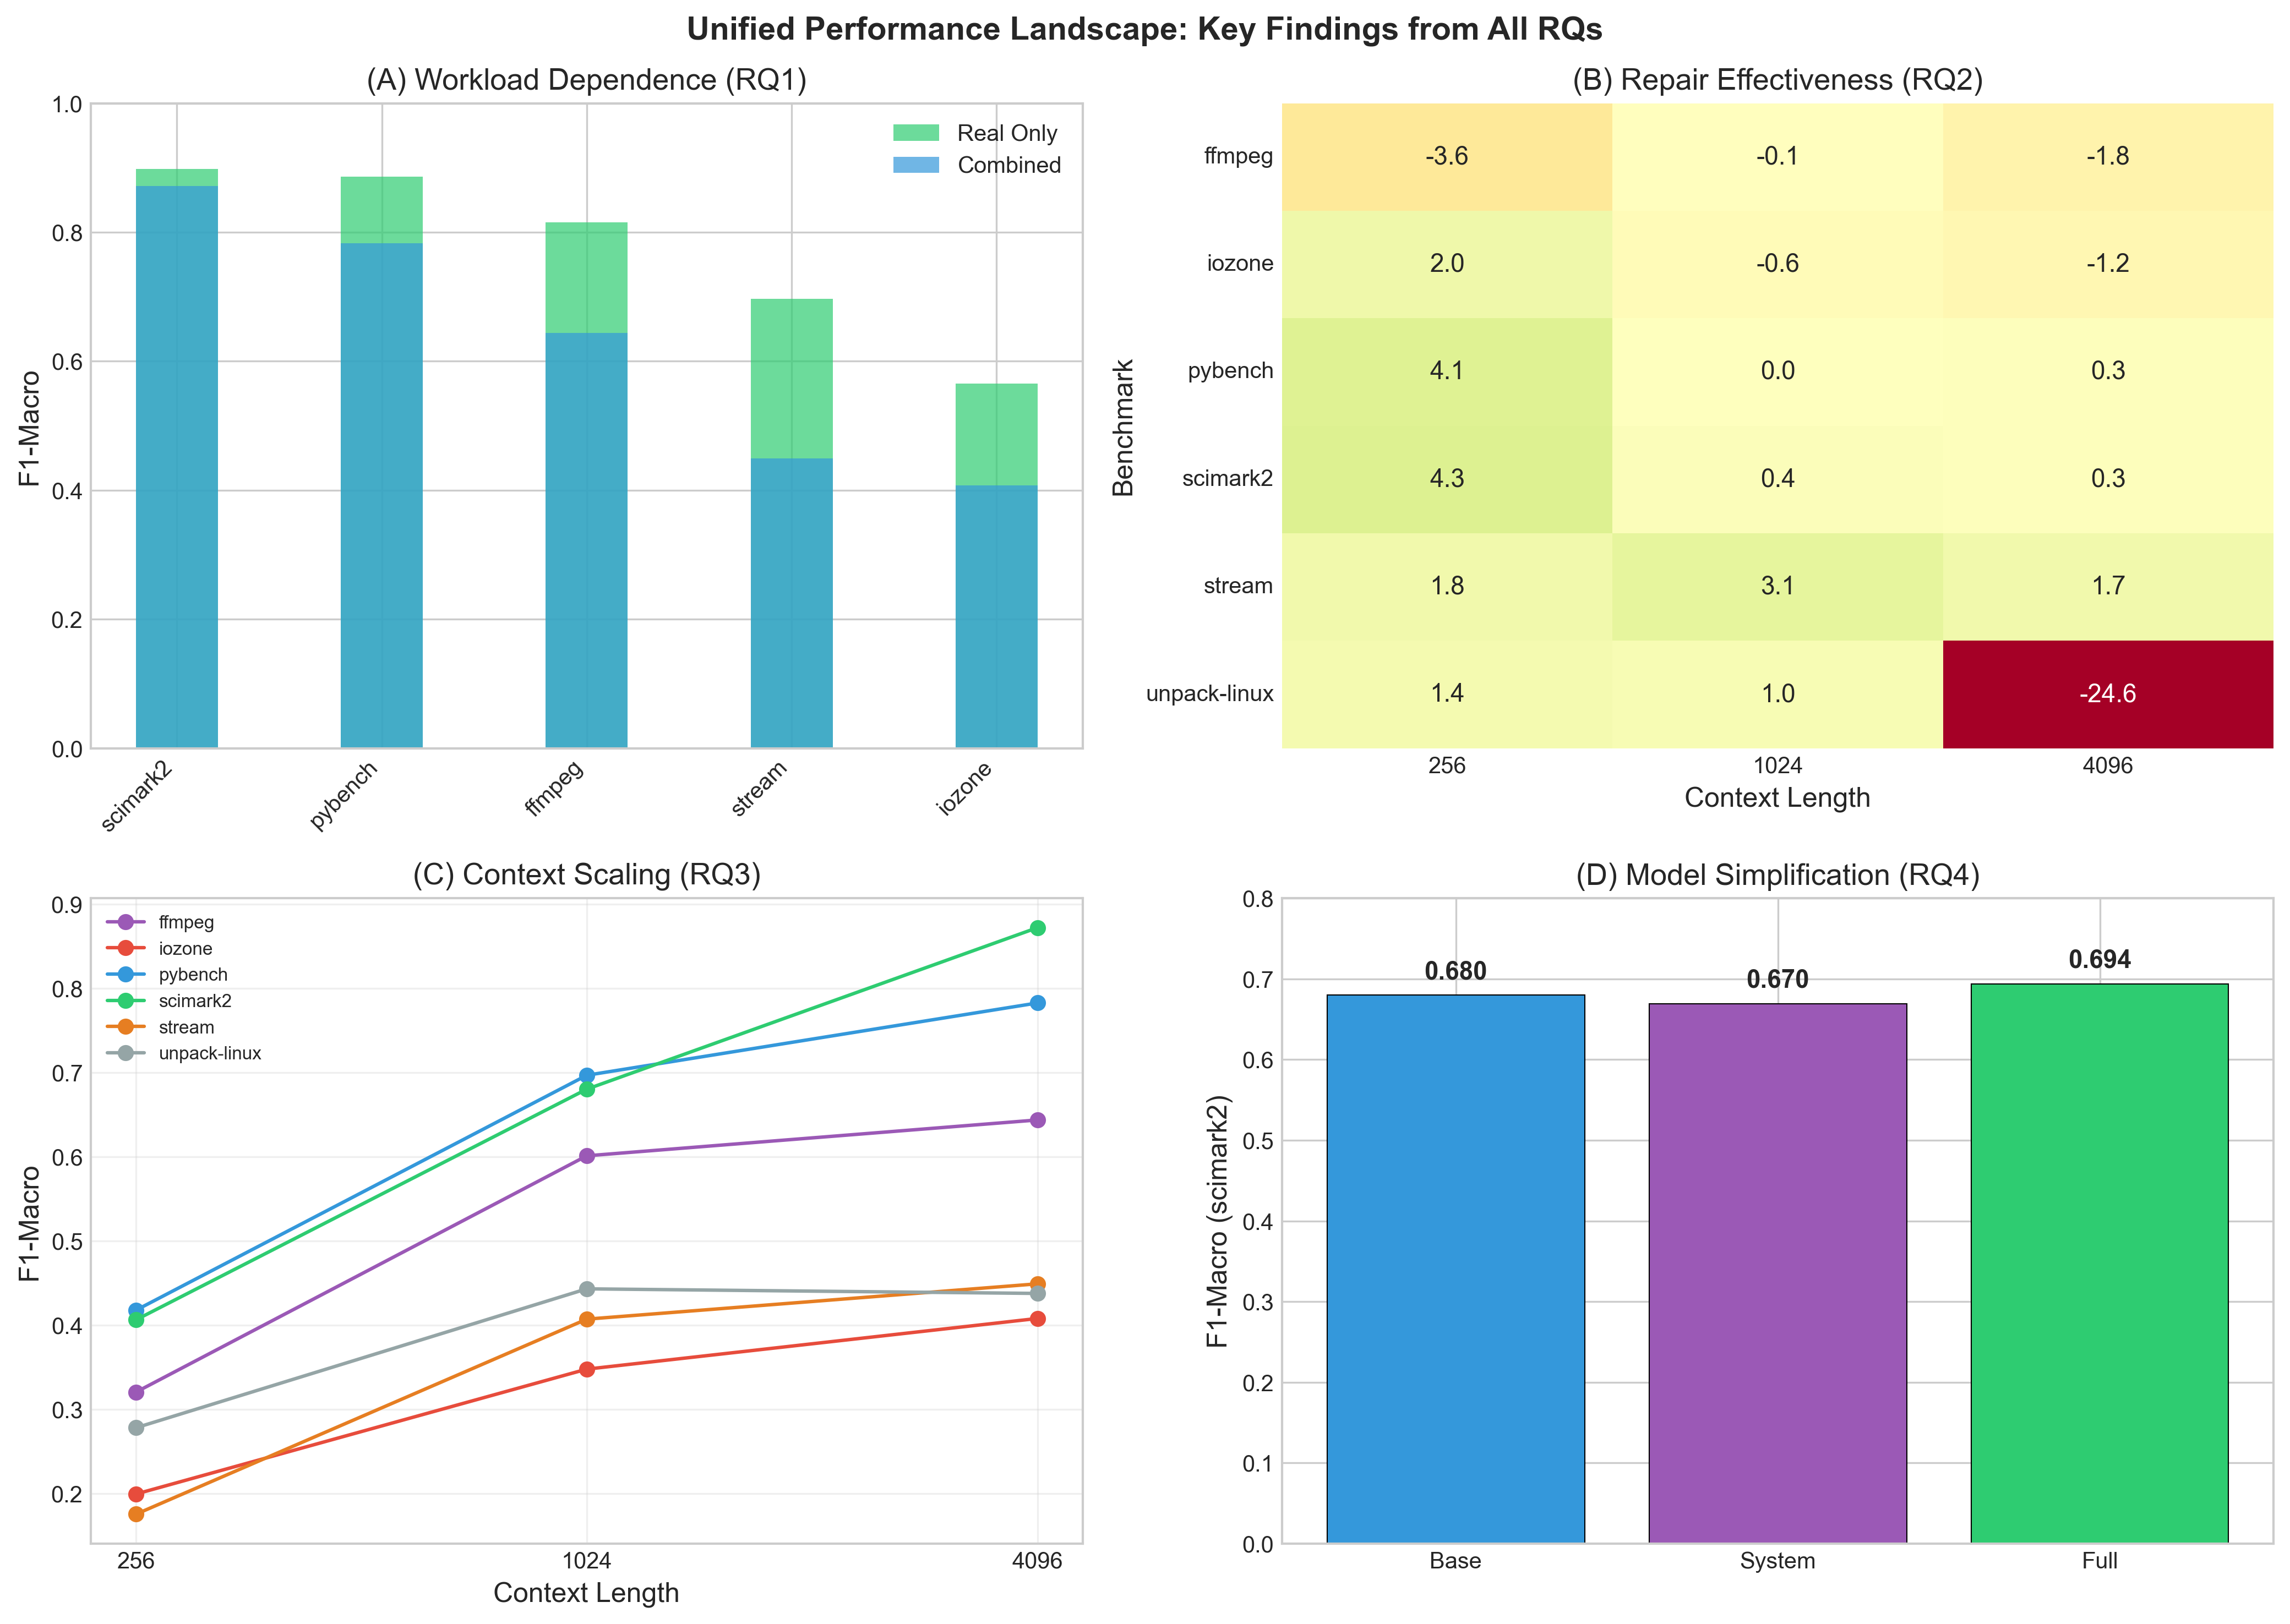
\includegraphics[width=0.95\columnwidth]{figures/cross_rq_plot12_unified_landscape.png}
% \caption{Unified Performance Landscape showing key findings from all four research questions. (A) Workload Dependence (RQ1): scimark2 and pybench achieve near-parity with real data, while I/O-heavy workloads show significant degradation. (B) Repair Effectiveness (RQ2): Constraint-guided repair provides consistent improvements, especially at shorter context lengths. (C) Context Scaling (RQ3): All benchmarks benefit from longer context, with scimark2 showing +46.6\% improvement from L=256 to L=4096. (D) Model Simplification (RQ4): Base 2-channel model achieves 97\% of Full 6-channel performance for scimark2.}
% \label{fig:unified-landscape}
% \end{figure}

% \subsection{Workload-Dependent Synthetic Data Quality}\label{subsec:workload-dependent-synthetic-data-quality}

% Our results reveal that synthetic data quality is fundamentally workload-dependent, with deterministic, structured workloads benefiting substantially more than non-deterministic I/O-heavy workloads. The scimark2 benchmark exemplifies this pattern: at L=4096, synthetic augmentation achieves 87.2\% F1-Macro, only 2.6 percentage points below the real-only baseline (89.8\%). This near-parity demonstrates that diffusion models \textit{can} generate production-quality synthetic kernel traces when three conditions are met: (i) the workload exhibits deterministic execution patterns, (ii) the diffusion model is trained with sufficient temporal context (L=4096), and (iii) constraint-guided repair is applied to ensure structural validity.

% In contrast, I/O-heavy benchmarks (stream, iozone, unpack-linux) show significant degradation (25--51\% at L=256, 25--36\% at L=4096), indicating that non-deterministic I/O patterns remain fundamentally challenging for current diffusion-based generation approaches. This workload dependence likely stems from the stochastic nature of I/O operations: filesystem caching, network latency, and device scheduling introduce variability that diffusion models struggle to capture faithfully. Deterministic workloads like scimark2, by contrast, follow predictable computation patterns that align well with the diffusion model's learned temporal dependencies.

% This finding has immediate practical implications. Organizations seeking to augment training data should first characterize their target workload: if it resembles scimark2 (numerical computation, deterministic loops, structured phases), synthetic augmentation is viable with minimal quality loss. If it resembles stream or iozone (intensive I/O, non-deterministic timing), synthetic data should be used cautiously, perhaps only for non-critical applications like testing or fuzzing where approximate behavior suffices.

% \subsection{The Dominant Role of Context Length}\label{subsec:the-dominant-role-of-context-length}

% Context length emerges as the single most important factor for synthetic data quality, with L=4096 doubling average performance (+104\% relative gain) compared to L=256. This universal improvement across all benchmarks---from +16.0\% (unpack-linux) to +46.6\% (scimark2)---demonstrates that kernel traces contain long-range dependencies spanning hundreds to thousands of events. Short context windows (L=256) fail to capture these dependencies, resulting in synthetic traces that lack coherent temporal structure.

% The scimark2 result is particularly illuminating: increasing from L=256 (40.6\% F1) to L=4096 (87.2\% F1) yields a +46.6 percentage point gain, transforming synthetic data from unusable to production-viable. This dramatic improvement suggests that numerical computation workloads have especially long-range dependencies---likely corresponding to nested loops, recursive function calls, and multi-phase algorithms that span thousands of system calls. The diffusion model's ability to capture these patterns at L=4096 explains why scimark2 achieves near-parity with real data.

% Importantly, even challenging I/O workloads benefit substantially from longer context. Stream improves by +27.4\% (+156\% relative), iozone by +20.9\% (+105\% relative), despite remaining below 50\% absolute F1. This suggests that context length is a \textit{necessary but not sufficient} condition for high-quality synthetic generation: it helps all workloads, but only deterministic workloads reach production-viable quality.

% From a practical deployment perspective, these results provide clear guidance: L=4096 should be the minimum context length for any synthetic trace generation system. The 2$\times$ performance improvement justifies the increased computational cost (approximately 16$\times$ memory, 4$\times$ training time). Organizations with sufficient resources should explore even longer contexts (L=8192, L=16384) to further improve quality, particularly for complex workloads.

% \subsection{Constraint-Guided Repair as Engineering Best Practice}\label{subsec:constraint-guided-repair-as-engineering-best-practice}

% Constraint-guided repair demonstrates consistent but modest improvements, with 80\% of configurations showing positive gains (+0.3\% to +4.3\%). While the average improvement (+0.9\%) is small compared to context length effects (+104\%), repair provides two critical benefits that justify its adoption as a standard engineering practice.

% First, repair \textit{guarantees} structural validity. Even when F1 gains are minimal, repair ensures 100\% valid event transitions and correct CPU affinity, which is essential for applications requiring hard constraints (e.g., trace replay, deterministic debugging). This guarantee is valuable beyond downstream task performance: it enables use cases where invalid traces would cause system failures or incorrect analysis.

% Second, repair is most effective precisely where it is most needed. At L=256, where diffusion models produce more constraint violations, repair provides the largest gains (+1.5\% average relative improvement). At L=4096, where the diffusion model already captures most structural patterns, repair provides smaller but still positive gains (+0.5\% average). This complementary relationship suggests that repair and longer context work synergistically: context length improves overall quality, while repair fixes residual violations.

% The practical recommendation is straightforward: always apply constraint-guided repair. The computational cost is negligible (greedy forward pass, no model retraining), the implementation is simple (learned transition rules + validity checks), and the benefits are consistent (80\% success rate). Even in cases with minimal F1 improvement, the validity guarantee alone justifies adoption.

% \subsection{Cost-Effective Model Simplification}\label{subsec:cost-effective-model-simplification}

% The ablation study reveals a surprising finding: simpler diffusion models (Base: 2 channels) achieve within 1--3\% of complex models (Full: 6 channels) while requiring only 33\% of computational resources. For ffmpeg and pybench, the Base model actually \textit{outperforms} the Full model (61.8\% vs 60.9\%, 71.3\% vs 71.2\%), suggesting that additional channels (cpu, tid, comm, ret) introduce noise rather than signal for these workloads.

% Only scimark2 shows a clear benefit from the Full model (+0.9\% over Base), likely because semantic metadata (comm, ret) helps capture program structure in deterministic numerical workloads. This workload-specific channel importance mirrors the broader pattern observed in RQ1: structured workloads benefit from richer modeling, while I/O-heavy workloads do not.

% From a cost-benefit perspective, these results suggest a tiered deployment strategy: (i) start with the Base model (event + dt) for all workloads, achieving 95--98\% of Full model quality with 3$\times$ lower cost; (ii) upgrade to the Full model only for deterministic, structured workloads where the +1\% gain justifies the computational overhead; (iii) allow downstream users to flexibly choose predictor channels based on their application needs, since predictor configuration has minimal impact (1--3\% variation) within each diffusion model.

% This finding challenges the common assumption that more data is always better. For synthetic trace generation, \textit{event timing patterns} (captured by the 2-channel Base model) appear to be the dominant signal, with system and semantic metadata providing marginal value for most workloads. This insight can guide future research toward more efficient diffusion architectures that prioritize temporal modeling over channel diversity.

% \subsection{Practical Applications Beyond F1-Macro}\label{subsec:practical-applications-beyond-f1-macro}

% While F1-Macro degradation limits synthetic data's utility for rare event prediction, secondary metrics reveal valuable alternative applications. F1-Weighted and Accuracy remain high (86--97\%) across all configurations, indicating that models trained on synthetic data perform well on \textit{common} events even when struggling with rare events. More encouragingly, Top-5 and Top-10 accuracy are consistently excellent (96--99.8\%), demonstrating that even when the top prediction is incorrect, the model captures plausible alternatives within a small set of candidates. This pattern suggests that synthetic data's value extends beyond exact prediction to diverse scenario generation.

% This high Top-K accuracy enables several practical use cases where exact prediction is less critical than diverse scenario generation:

% \textbf{Software testing and fuzzing.} Synthetic traces can generate diverse execution scenarios for testing system behavior under varied conditions. The ability to produce multiple plausible event sequences (high Top-K accuracy) is more valuable than predicting a single next event with perfect accuracy. Organizations can use synthetic data to expand test coverage, explore edge cases, and validate system robustness without collecting extensive real traces. The 86--97\% accuracy on common events ensures that typical system behavior is faithfully represented, while the diversity of plausible alternatives enables comprehensive testing of corner cases.

% \textbf{Privacy-preserving analysis.} Organizations can share synthetic kernel traces for collaborative research or debugging without exposing sensitive real system data. This is particularly valuable when real traces contain proprietary workload patterns, security-sensitive information, or personally identifiable data. The 86--97\% accuracy on common events ensures that synthetic traces preserve typical system behavior while protecting privacy. The 2$\times$ dataset size benefit can significantly reduce data collection infrastructure costs while maintaining high fidelity for collaborative analysis.

% \textbf{Development and prototyping.} Developers can use synthetic data to train and validate monitoring tools, anomaly detectors, or performance analyzers when real production data is unavailable or expensive to collect. The 2$\times$ dataset size benefit can significantly reduce data collection infrastructure costs while maintaining 86--97\% accuracy on typical system behavior, enabling faster development cycles and lower operational overhead.

% \textbf{Edge case exploration.} The ability to generate plausible alternatives (high Top-K accuracy) allows systematic exploration of rare execution paths that may not appear frequently in real traces but are critical for robustness testing. This is valuable for security analysis, fault injection testing, and corner case validation.

% These alternative applications suggest that synthetic data's value extends beyond traditional supervised learning metrics. For practitioners, the recommendation is to match synthetic data usage to application requirements: use real data for rare event prediction (security anomaly detection), but leverage synthetic data for testing, privacy preservation, and development where approximate behavior suffices. When the primary goal is generating diverse scenarios for testing, achieving high accuracy on common events, or preserving privacy, synthetic data offers substantial practical value even for workloads with moderate F1-Macro degradation.

% \subsection{Implications for Future Research}\label{subsec:implications-for-future-research}

% Our findings identify several promising directions for improving diffusion-based synthetic trace generation:

% \textbf{Longer context lengths.} The universal benefit of L=4096 over L=256 (+104\% relative gain) suggests that even longer contexts (L=8192, L=16384) may further improve quality. Future work should explore sparse attention mechanisms (Longformer, BigBird) to make longer contexts computationally feasible, particularly for challenging I/O workloads that remain below 50\% F1 at L=4096.

% \textbf{Workload-specific architectures.} The stark performance difference between deterministic (scimark2: 87.2\%) and non-deterministic (stream: 44.9\%) workloads suggests that one-size-fits-all diffusion models may be suboptimal. Future research could develop specialized architectures for I/O-heavy workloads, perhaps incorporating explicit models of filesystem caching, device scheduling, or network latency.

% \textbf{Improved rare event modeling.} The gap between F1-Macro (59.9\% average) and F1-Weighted/Accuracy (93.7--93.8\%) indicates that current diffusion models underrepresent rare events. Techniques like class-balanced sampling, importance weighting, or adversarial training could help models better capture rare but critical events (errors, security events, anomalies).

% \textbf{Conditional generation.} Current models generate traces unconditionally. Future work could explore conditional diffusion models that generate traces with specific properties (duration, event distribution, workload type), enabling more targeted synthetic data generation for specific use cases.

% \textbf{Alternative generative models.} While diffusion models show promise, other generative approaches (flow matching, latent diffusion, autoregressive transformers) may offer better quality or efficiency trade-offs. Comparative studies across generative model families would help identify the optimal approach for kernel trace synthesis.

